\section{Attachements}
\subsection{Vorbereitung}
In der Versuchsvorbereitung wurden mit Matlab der IIR-Filterentwurf untersucht. Dabei wurden die zwei Filtertypen, elliptisch und Chebychev mit den Spezifikationen siehe Aufgabenbeschreibung simuliert. Für die spätere Implementierung auf einen DSP wurden die resultierenden Übertragungsfunktionen auf Systeme 2. Ordnung reduziert. Die Verstärkungsfaktor g wird dabei auf die einzelnen Systeme 2. Ordnung gleichmäßig aufgeteilt.
\subsubsection{Attachement A}

Die Filtercharakteristik Elliptisch, Chebychev sind in der Allgemeinen und in der Kaskadenstruktur in ihrem Amplitudengang in den nachfolgenden Abbildungen Dargestellt.

\begin{figure}[h]
\centering
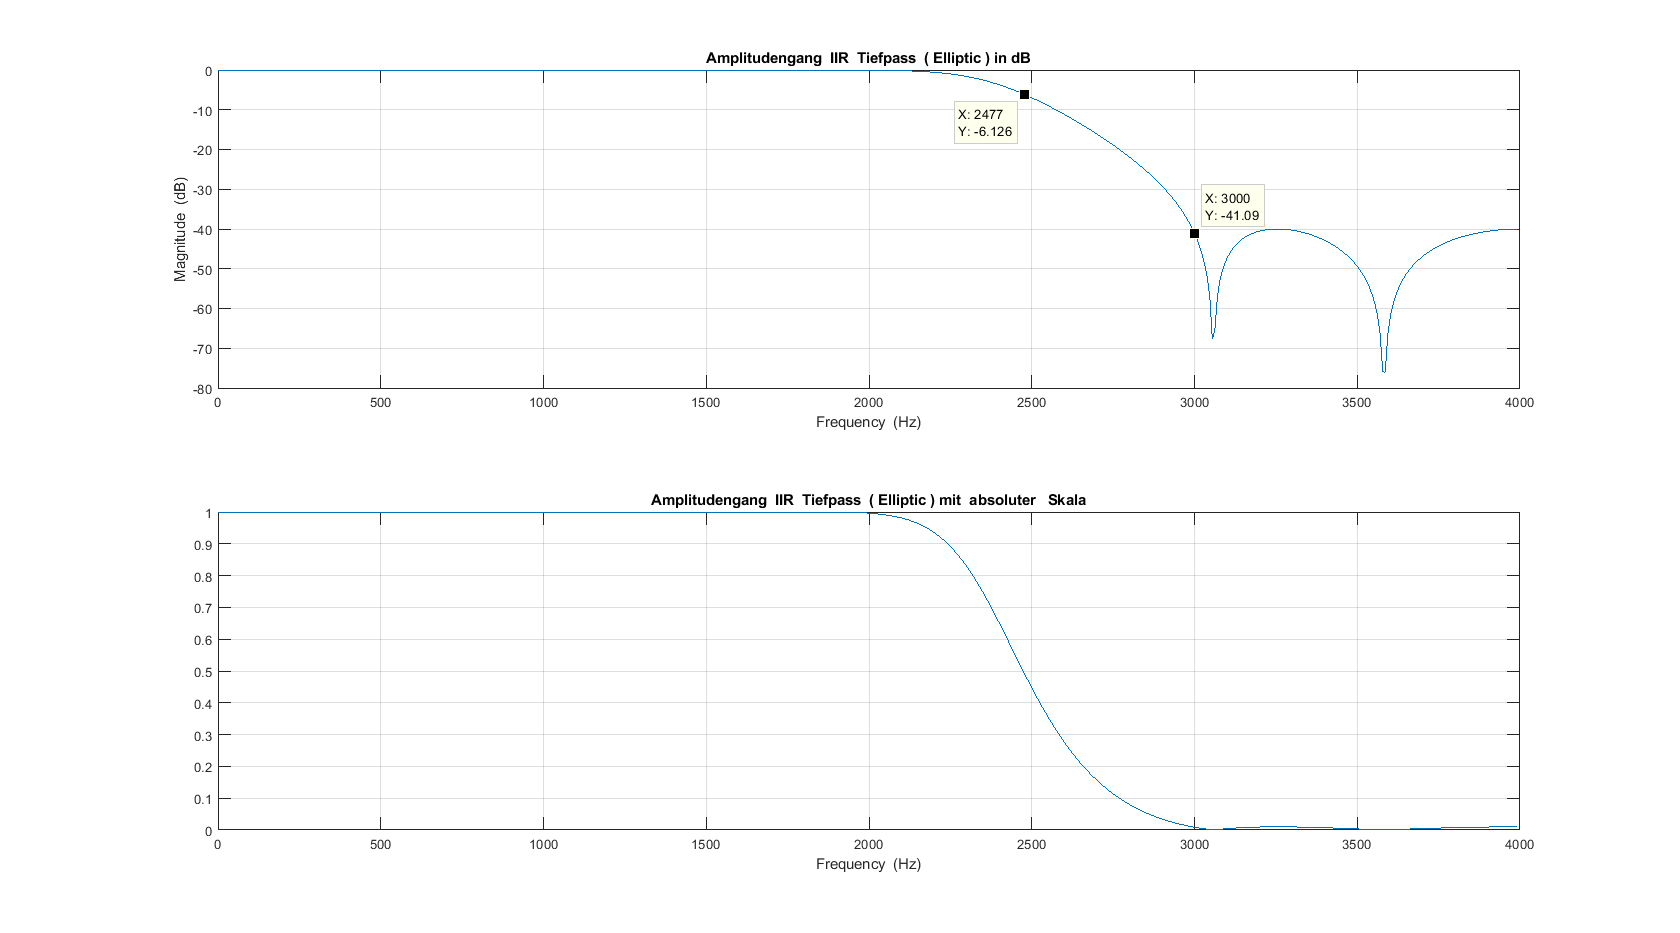
\includegraphics[width=0.7\linewidth]{Bilder/Attachment_A_ELLIP}
\caption{IIR-Filter: Elliptischer-Filtertyp - Amplitudengang}
\label{fig:Attachment_A_ELLIP}
\end{figure}
\noindent Amplitudengang des elliptischen Filtercharakteristik. Die maximale und minimale Dämpfung wird sowohl im Passband als auch im Stopband eingehalten.

\clearpage

\begin{figure}[h]
	\centering
	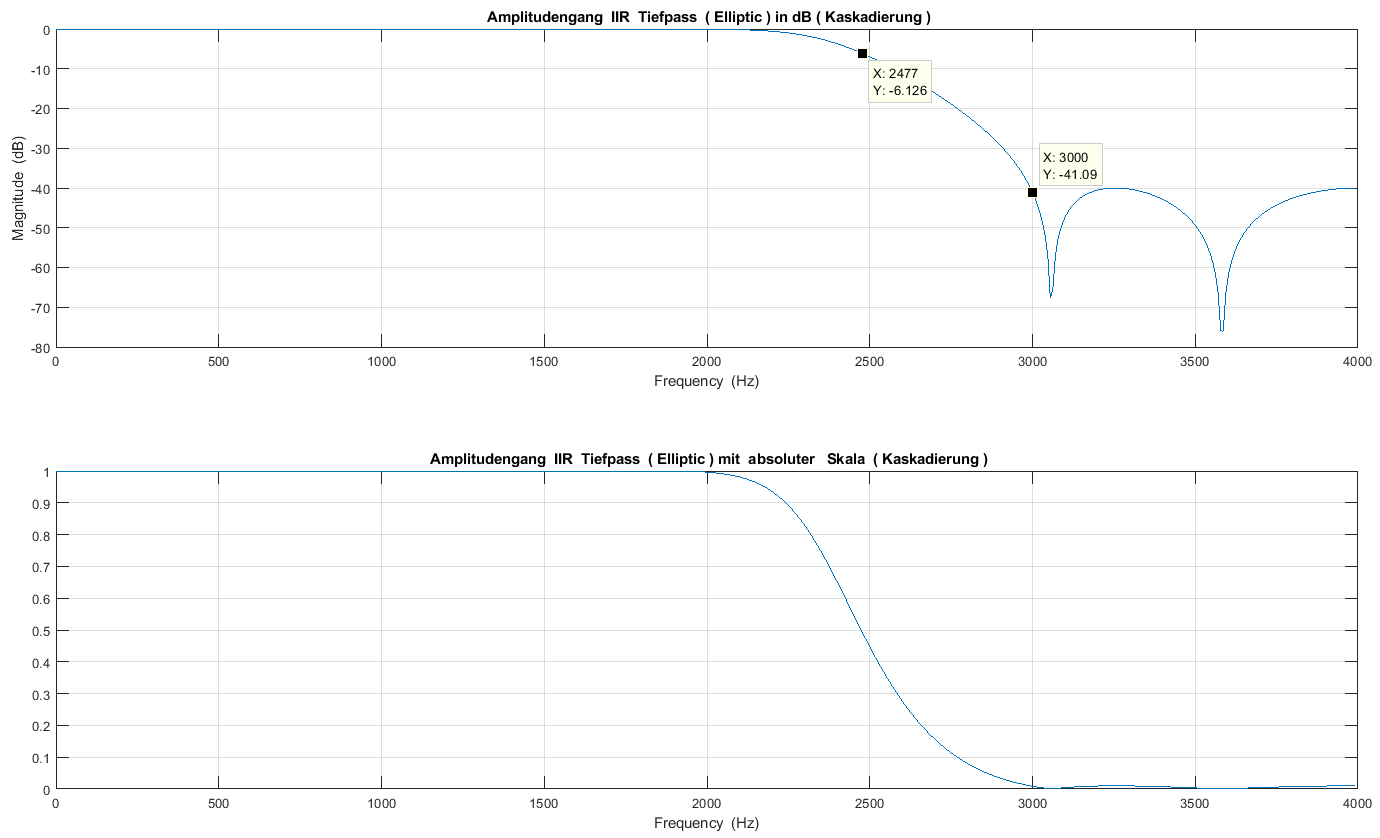
\includegraphics[width=0.7\linewidth]{Bilder/Attachment_A_ELLIP_KASKADE}
	\caption{IIR-Filter: Elliptischer-Filtertyp Kaskadenstruktur - Amplitudengang}
	\label{fig:Attachment_A_ELLIP_KASKADE}
\end{figure}
\noindent Die kaskadierte Form des elliptischen Filter zeigt den gleichen Verlauf auf wie die allgemein Form auf.

\begin{figure}[h]
\centering
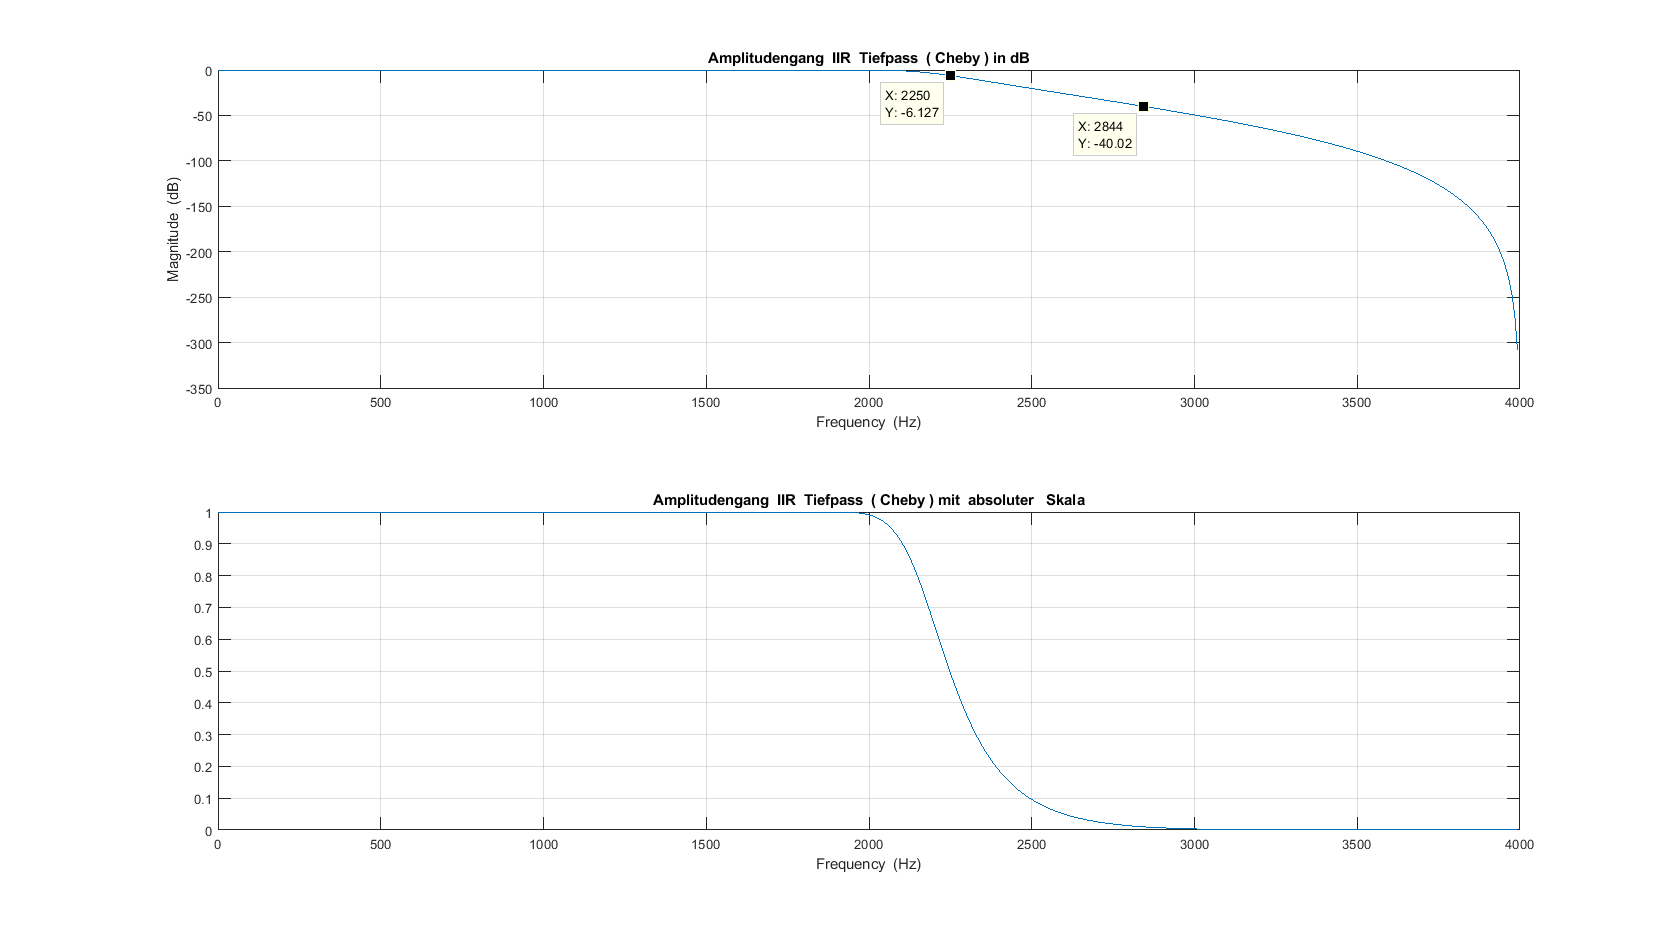
\includegraphics[width=0.7\linewidth]{Bilder/Attachment_A_CHEBY}
\caption{IIR-Filter: Chebychev-Filtertyp - Amplitudengang}
\label{fig:Attachment_A_CHEBY}
\end{figure}
\noindent Amplitudenverlauf des Chebychev Filtertyp. Die maximale Sperrdämpfung ist im Vergleich zum elliptischen Filtertyp stärker und steigt nicht mehr im Auflösungsbereich an.

\clearpage

\begin{figure}[h]
\centering
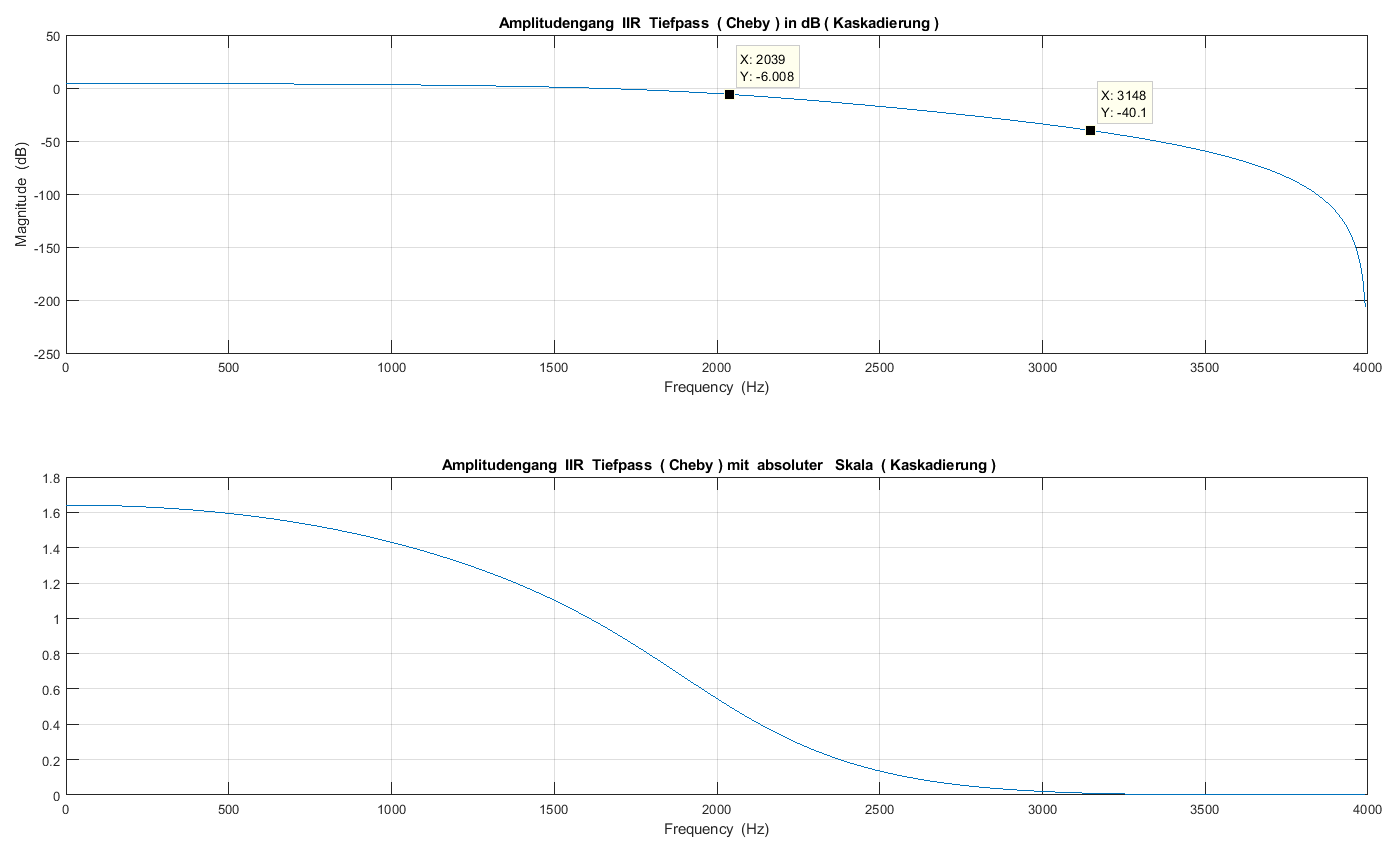
\includegraphics[width=0.7\linewidth]{Bilder/Attachment_A_CHEBY_KASKADE}
\caption{IIR-Filter: Chebychev-Filtertyp Kaskadenstruktur - Amplitudengang}
\label{fig:Attachment_A_CHEBY_KASKADE}
\end{figure}
\noindent Bei der kaskadierten Form des Chebychev-Filtertyp ist der Ripple im Passband stärker als in der allgemeinen Form und ist nicht mehr in den Spezifikationen von 0.1 db.\\

\noindent Im nachfolgenden Listing ist ein Auszug des Matlabskript zur Bestimmung des Filter Koeffizienten und Umwandlung in Systeme 2. Ordnung. Als Hinweis sei hier nochmal erwähnt, dass der Verstärkungsfaktor g bei der Überführung in Systemform 2. Ordnung auf die Koeffizienten der einzelnen Stufen gleichmäßig verteilt wird, um einen Überlauf bei der Implementierung in die Hardware zu verhindern. In der hier eingesetzten Form der Biquad wird die Verstärkung auf die b-Koeffizienten skaliert. Zusätzlich müssen noch alle Koeffizienten auf Eins normiert werden. $b_{k_{normiert}} = b_{k} \cdot 32767$\\

\begin{figure}[h]
\centering
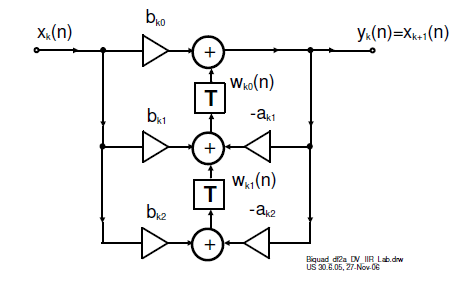
\includegraphics[width=0.7\linewidth]{Bilder/BIQUAD}
\caption{ Realisierung der k-ten Sektion 2er-Ordnung (BIQUAD)}
\label{fig:BIQUAD}
\end{figure}

\clearpage

\lstinputlisting[style=c, caption={IIR-Filter Matlab Skript}, label={lst:fir_2a_koeff}]{Code/IIR_Filter_koeffizienten.m}

\noindent Koeffizienten der Filtertypen: Elliptisch und Chebychev\\
Bei den Koeffizienten ist zu erkennen, dass mit einer elliptischen Implementierung zwei Biquads benötigt werden um die Spezifikationen zu erreichen. Mit der Chebychev Umsetzung werden drei Stages benötigt um diese zu erreichen.\\


\lstinputlisting[style=c, caption={IIR-Filter Koeffizienten elliptischer Typ als Tiefpass}, label={lst:fir_2a_koeff}]{Code/IIR_ellip_LP.h}

\lstinputlisting[style=c, caption={IIR-Filter Koeffizienten elliptischer Typ als Tiefpass}, label={lst:fir_2a_koeff}]{Code/IIR_cheby1_LP.h}

\clearpage

\subsubsection{Attachement B}
Implementierung eines Hochpassfilters mit elliptischer Filter-Charakteristik. Nachfolgend ist der Amplitudengang und die Filterkoeffizienten dargestellt.

\begin{figure}[h]
\centering
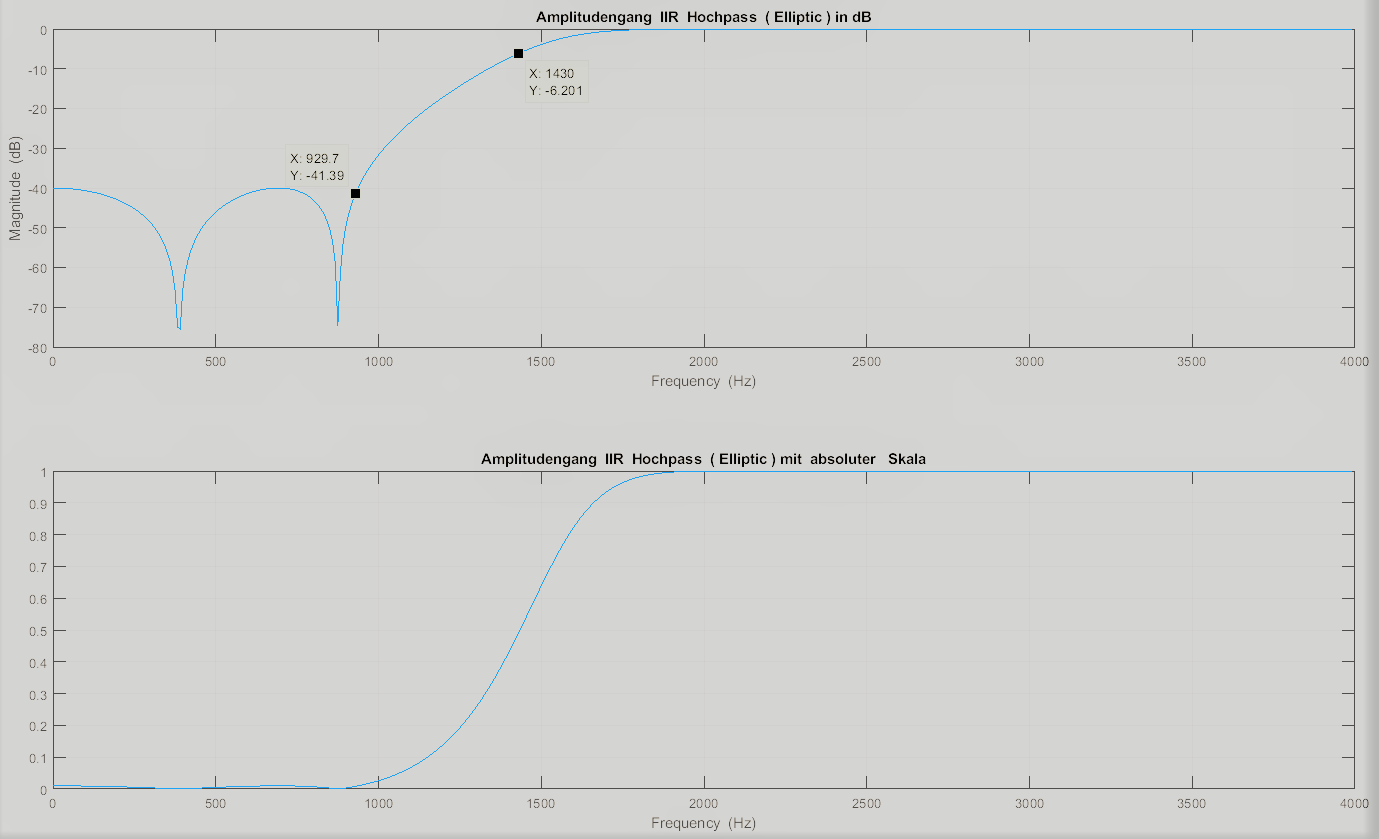
\includegraphics[width=0.7\linewidth]{Bilder/Attachment_B_ELLIP}
\caption{IIR-Filter: Chebychev-Filtertyp - Amplitudengang}
\label{fig:Attachment_B_ELLIP}
\end{figure}


\begin{figure}[h]
\centering
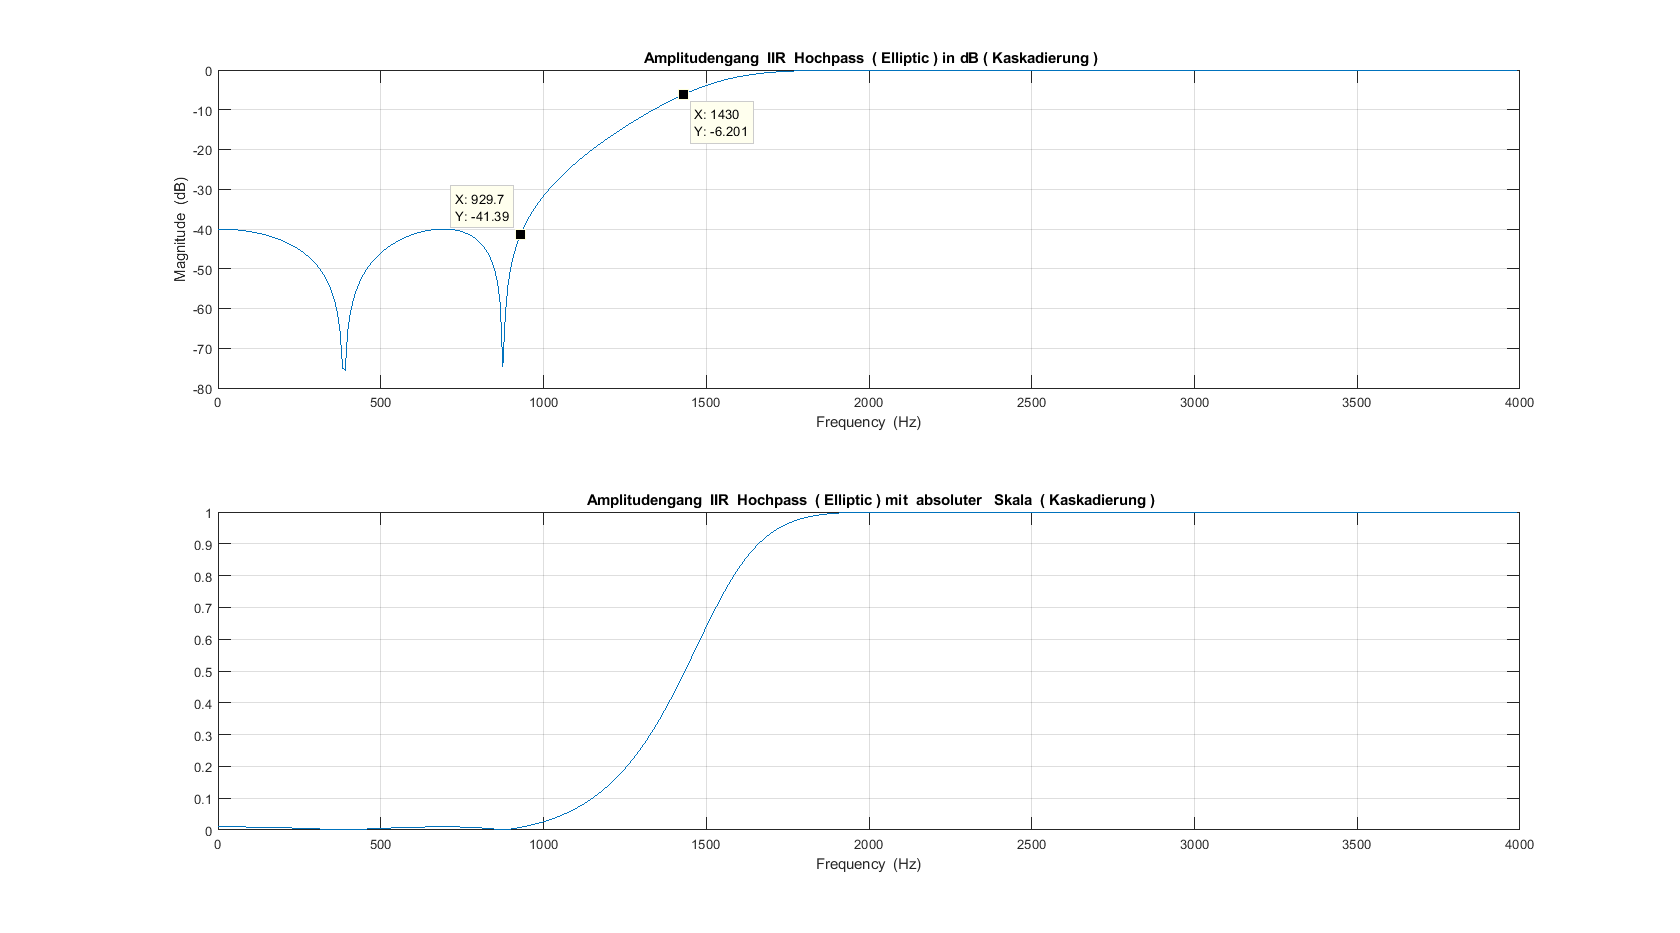
\includegraphics[width=0.7\linewidth]{Bilder/Attachment_B_ELLIP_KASKADE}
\caption{}
\label{fig:Attachment_B_ELLIP_KASKADE}
\end{figure}

\lstinputlisting[style=c, caption={IIR-Filter Koeffizienten elliptischer Typ als Hochpass}, label={lst:fir_2a_koeff}]{Code/IIR_ellip_HP.h}

\clearpage

\subsubsection{Attachement D}
Simulationsergebnisse im Zeitbereich der drei Filter (ellip LP, cheby LP und ellip HP)
\begin{figure}[h]
\centering
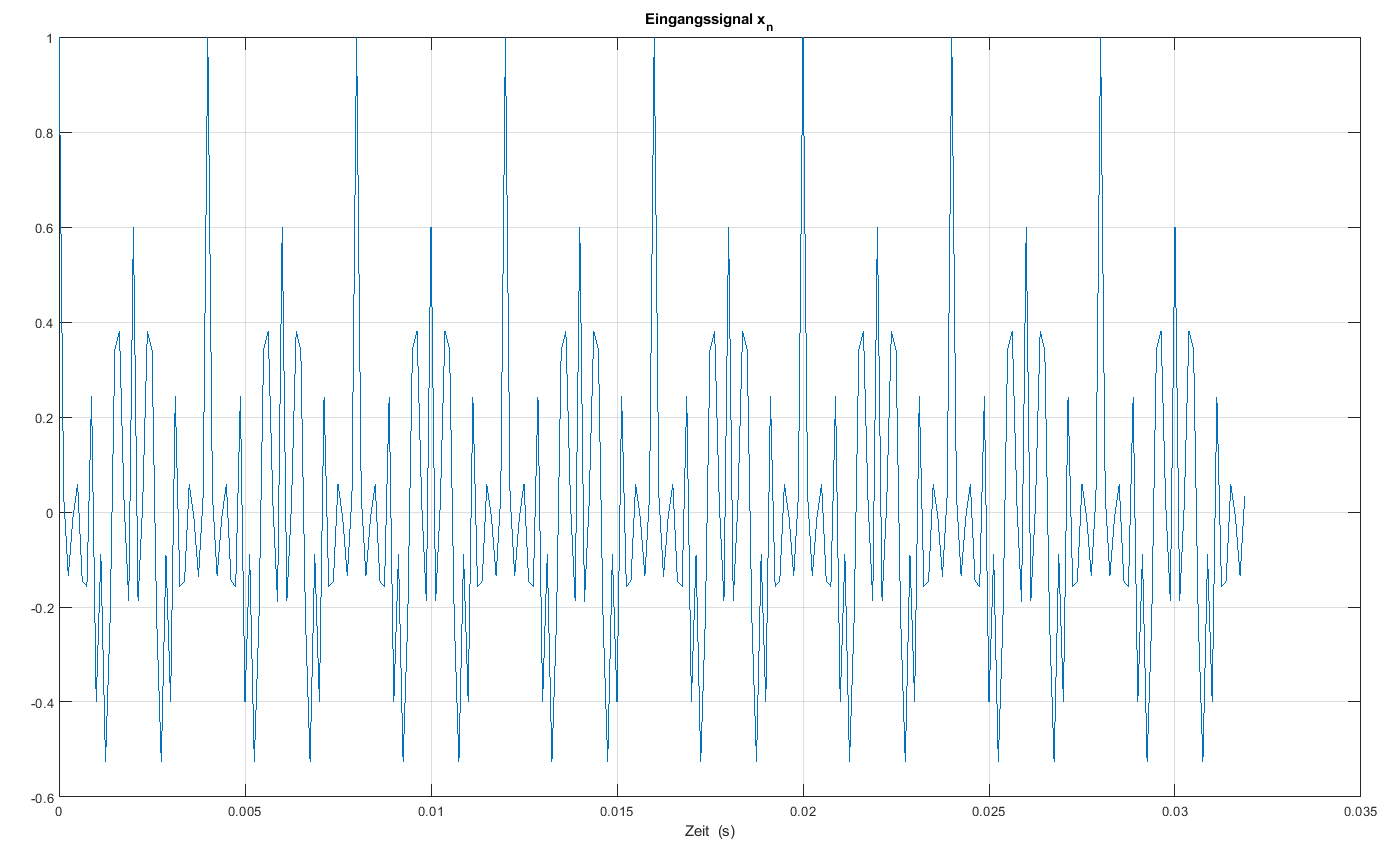
\includegraphics[width=0.7\linewidth]{Bilder/Attachment_D_Eingangszeitsignal}
\caption{$X_{n}$ Eingangs-Zeitsignal }
\label{fig:Attachment_D_Eingangszeitsignal}
\end{figure}

\begin{figure}[h]
\centering
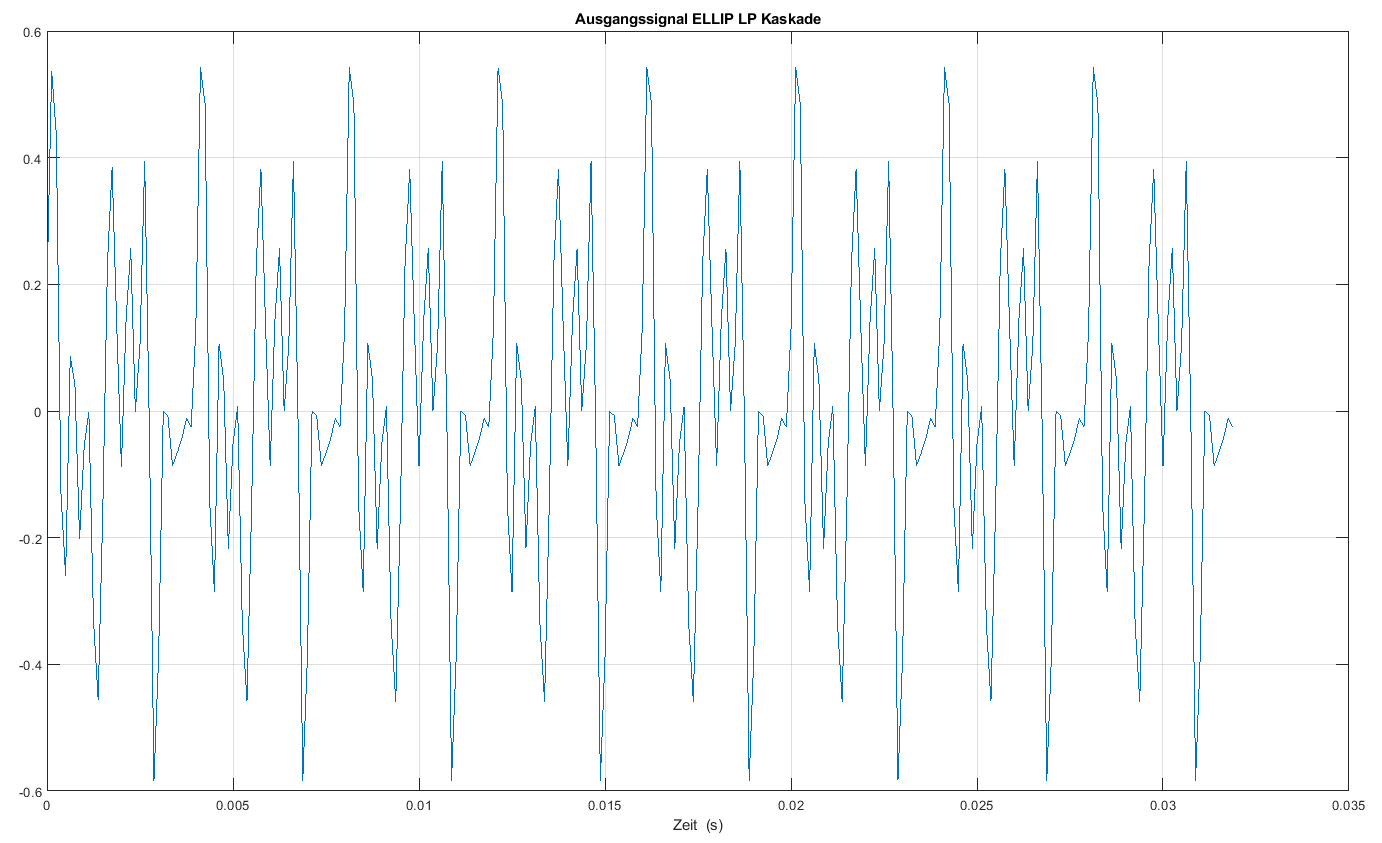
\includegraphics[width=0.7\linewidth]{Bilder/Attachment_D_Ausgangssignal_ellip_lp}
\caption{$Y_{n}$ Ausgangssignal kaskadierter Ellip-LP}
\label{fig:Attachment_D_Ausgangssignal_ellip_lp}
\end{figure}

\clearpage

\begin{figure}[h]
\centering
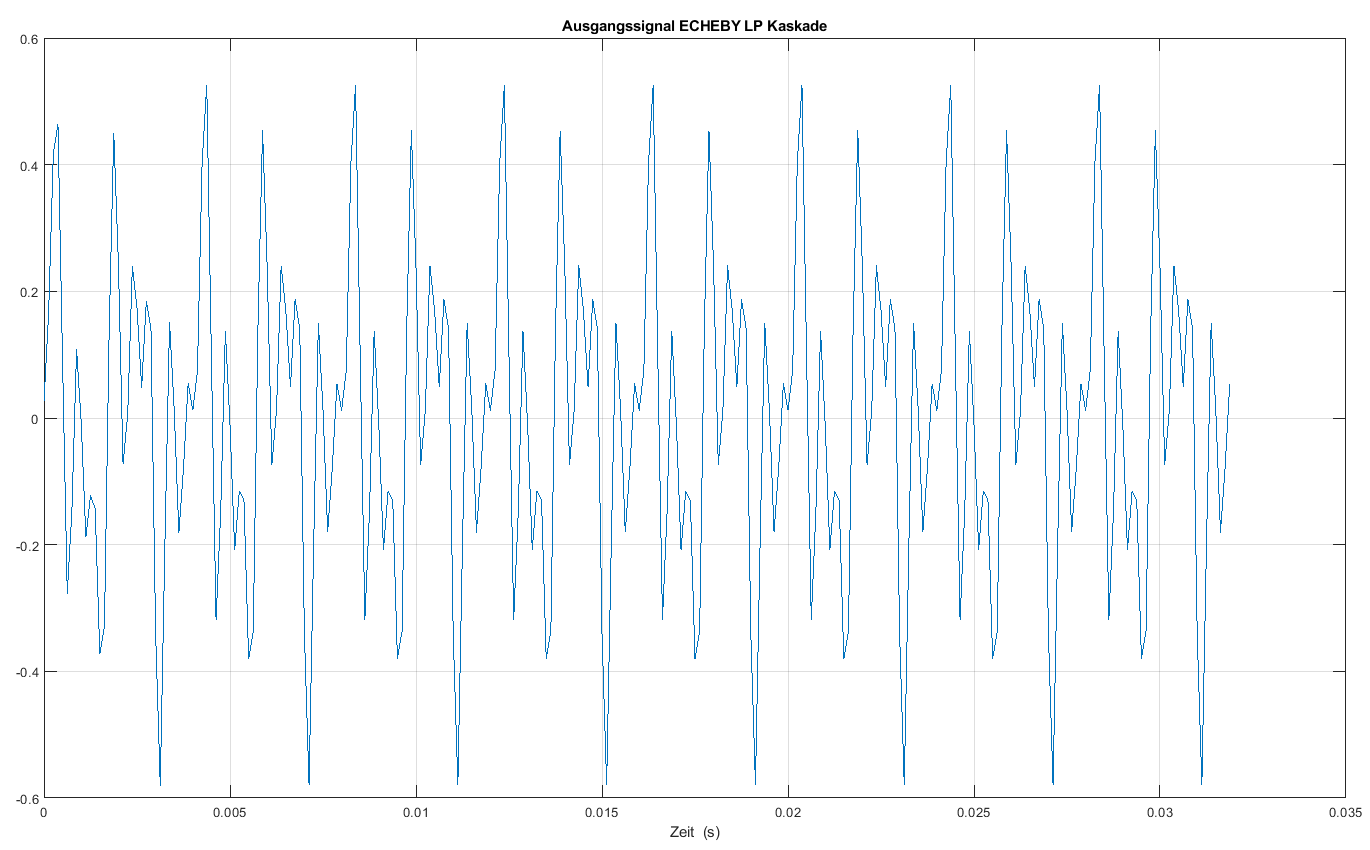
\includegraphics[width=0.7\linewidth]{Bilder/Attachment_D_Ausgangssignal_cheby_lp}
\caption{$Y_{n}$ Ausgangssignal kaskadierter Checby-LP}
\label{fig:Attachment_D_Ausgangssignal_cheby_lp}
\end{figure}

\begin{figure}[h]
\centering
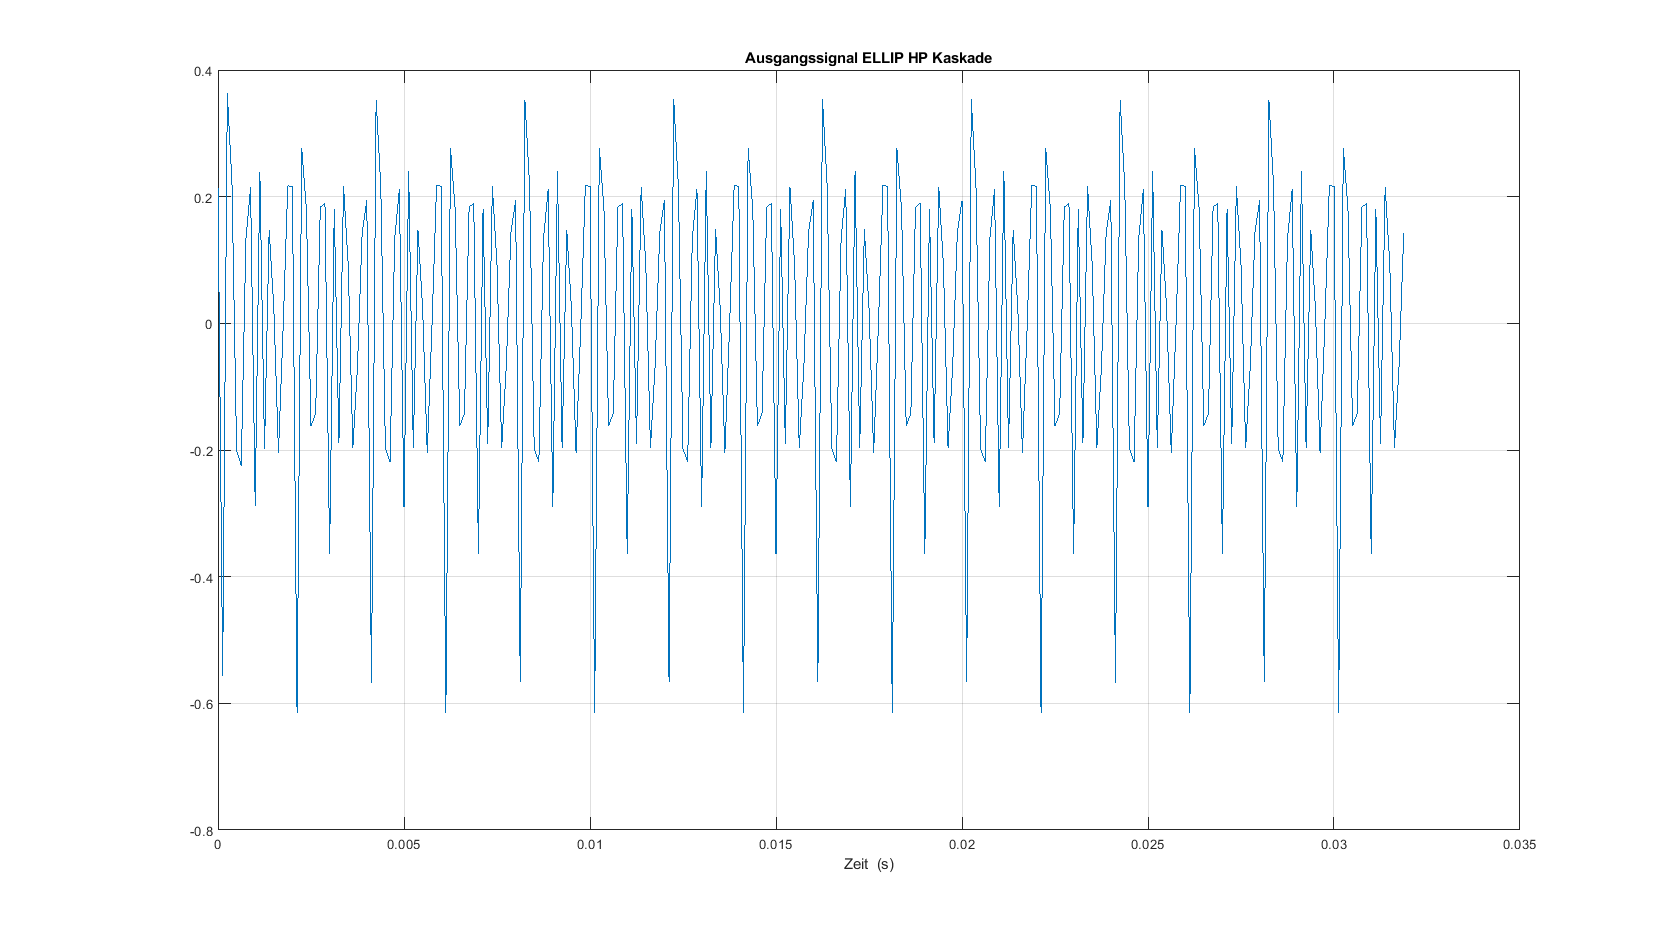
\includegraphics[width=0.7\linewidth]{Bilder/Attachment_D_Ausgangssignal_ellip_hp}
\caption{$Y_{n}$ Ausgangssignal kaskadierter Ellip-HP}
\label{fig:Attachment_D_Ausgangssignal_ellip_hp}
\end{figure}

\noindent Bei den Simulationsergebnissen im Zeitbereich kann die Filtereigenschaften sehr gut nach Tiefpass- und Hochpassverhalten erkannt werden.\\
Beim Cheby-LP kann im Zeitsignal die stärkere Dämpfung im Sperrband durch eine größere Unterdrückung der hohen Frequenzanteile gegenüber dem Ellip-LP bestätigt werden.

\clearpage

\subsubsection{Attachement E}
Frequenzspektrum der Zeitsignale vor und nach den Filtertypen.
\begin{figure}[h]
\centering
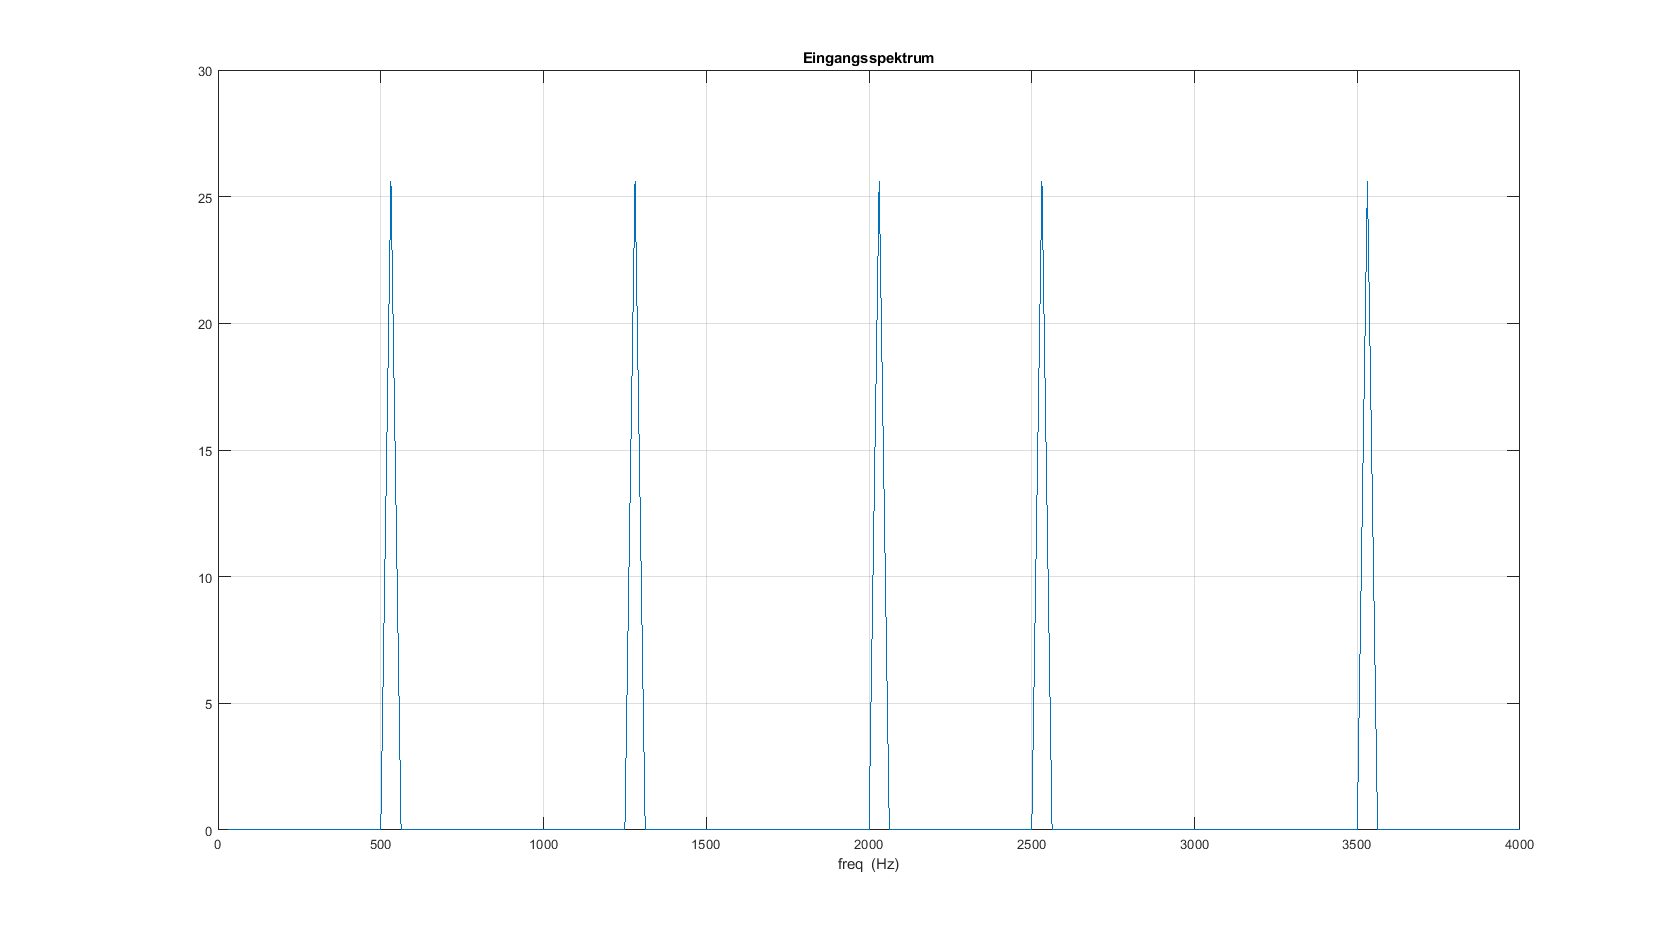
\includegraphics[width=0.7\linewidth]{Bilder/Attachment_E_Eingangsspektrum}
\caption{$X_{n}$ Frequenzspektrum des Eingangssignals}
\label{fig:Attachment_E_Eingangsspektrum}
\end{figure}

\begin{figure}[h]
\centering
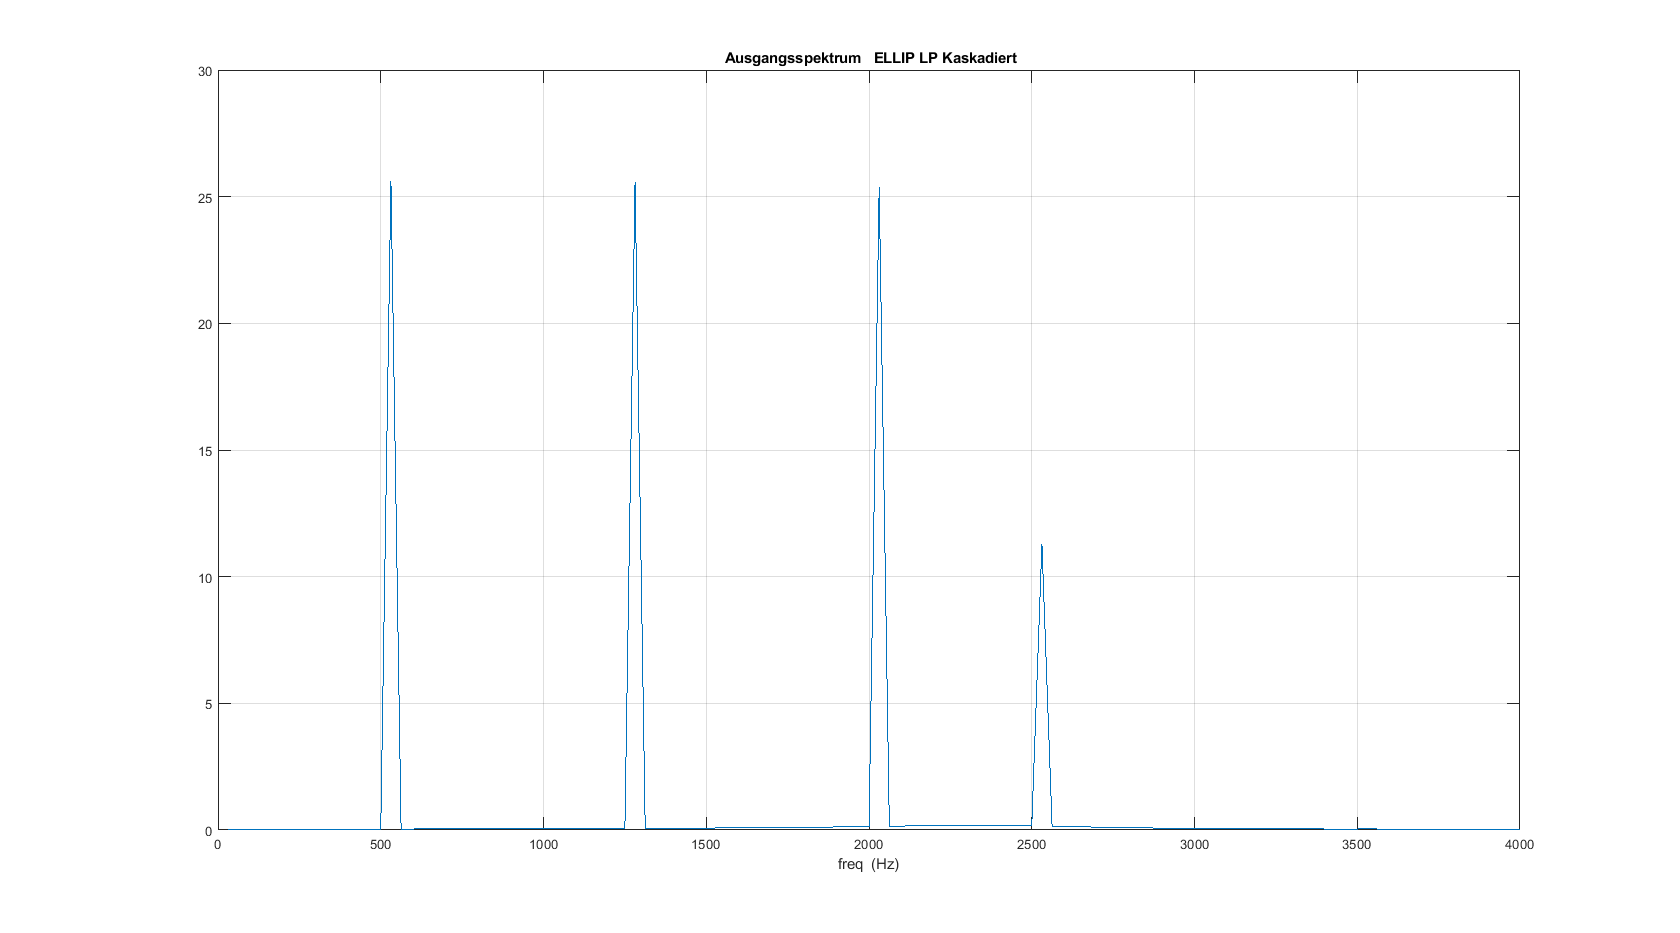
\includegraphics[width=0.7\linewidth]{Bilder/Attachment_E_ELLIP_LP_Spektrum}
\caption{$Y_{n}$ Ausgangs-Frequenzspektrum des kaskadierter Ellip-LP}
\label{fig:Attachment_E_ELLIP_LP_Spektrum}
\end{figure}

\newpage

\begin{figure}[h]
\centering
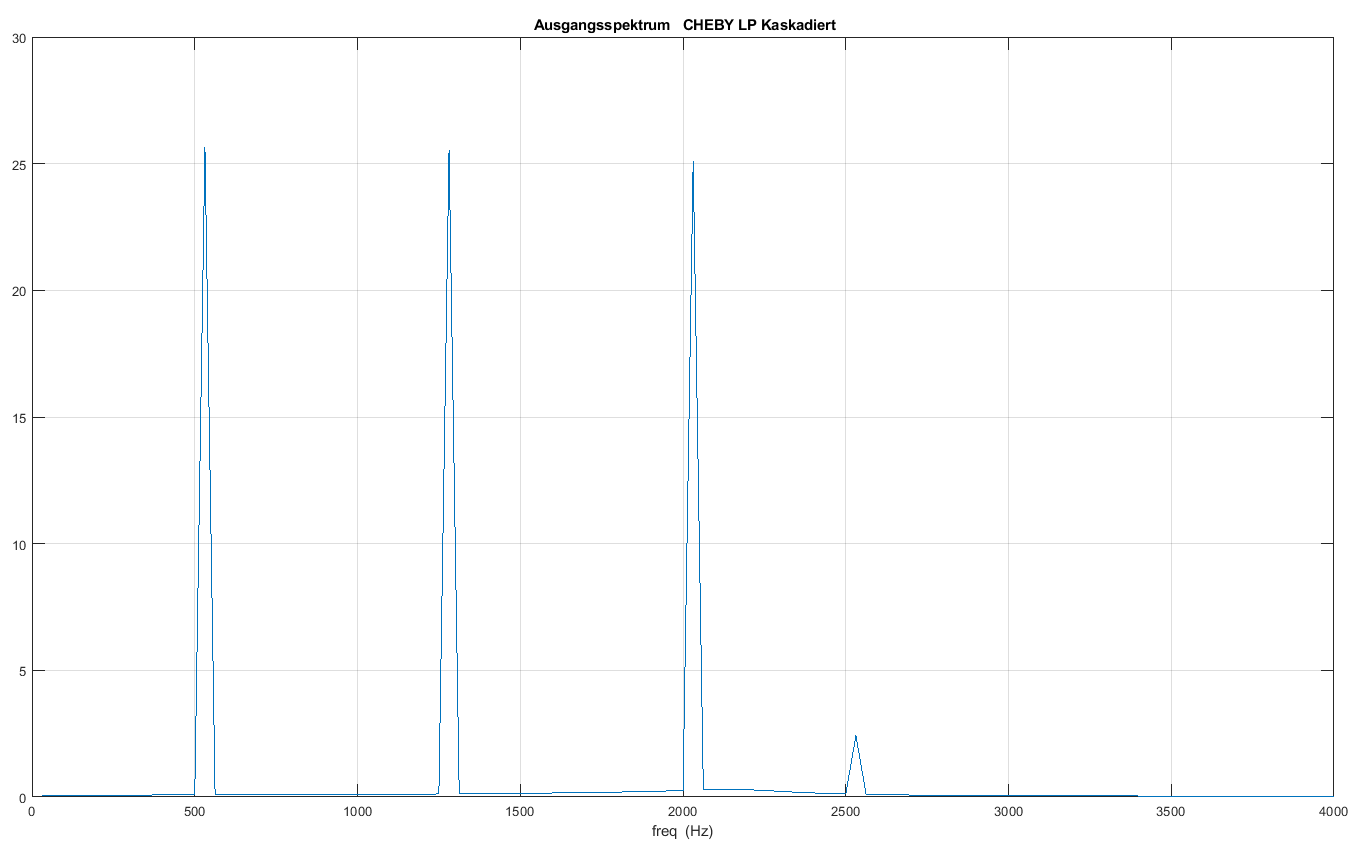
\includegraphics[width=0.7\linewidth]{Bilder/Attachment_E_CHEBY_LP_Spektrum}
\caption{$Y_{n}$ Ausgangs-Frequenzspektrum des kaskadierter Cheby-LP}
\label{fig:Attachment_E_CHEBY_LP_Spektrum}
\end{figure}

\begin{figure}[h]
\centering
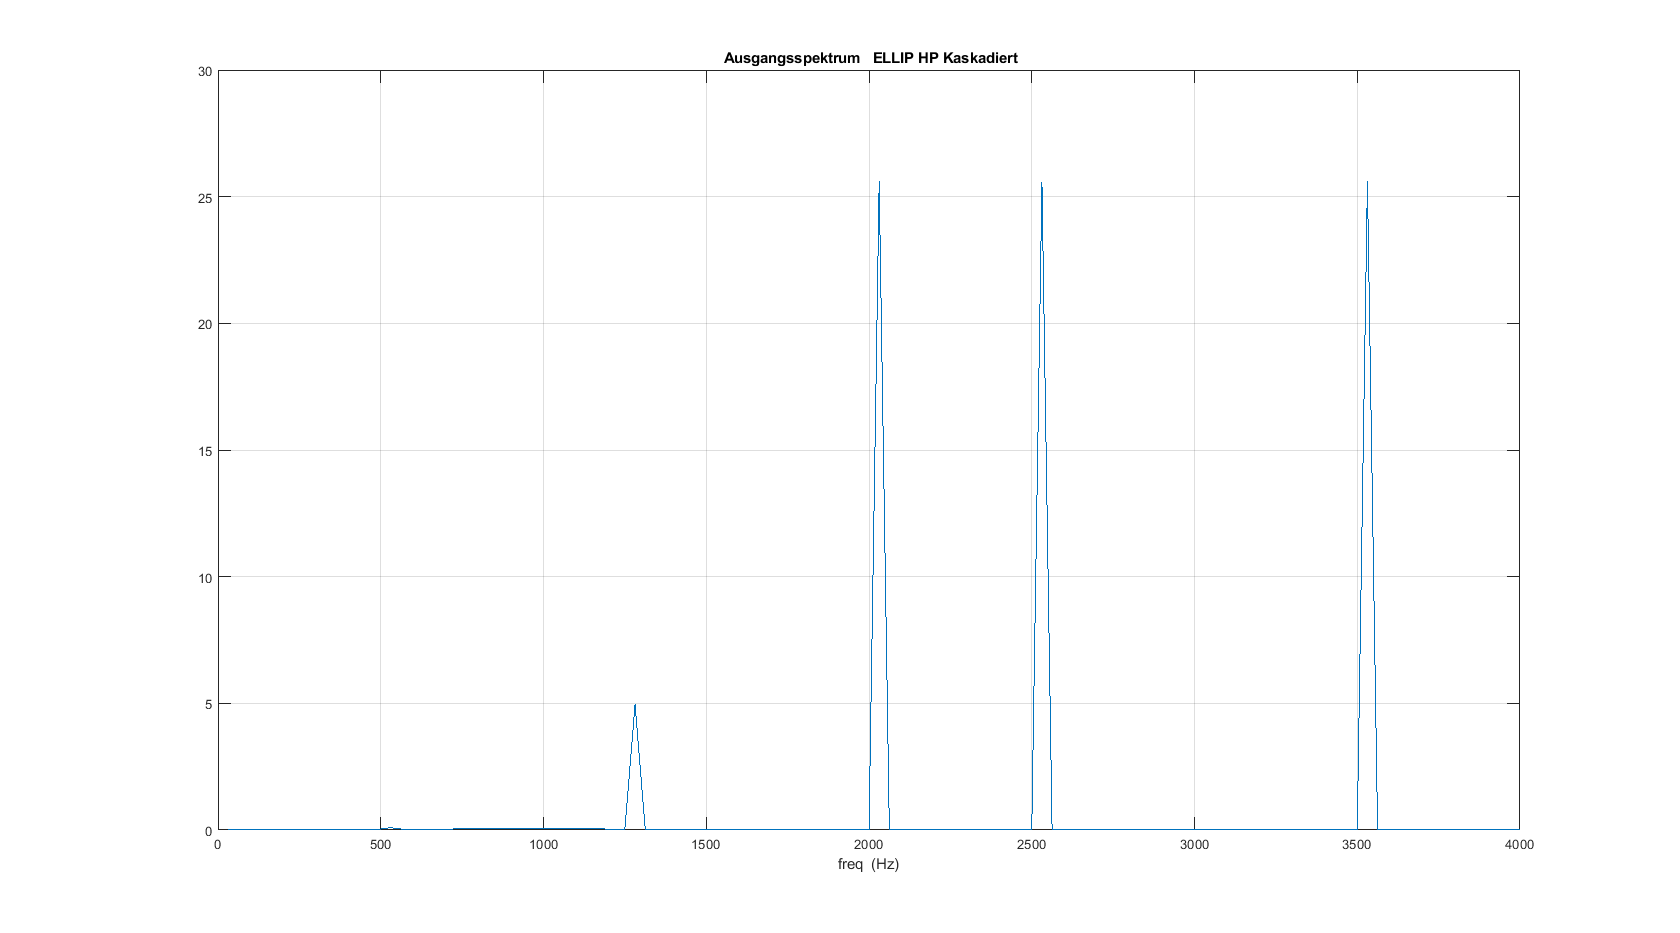
\includegraphics[width=0.7\linewidth]{Bilder/Attachment_E_ELLIP_HP_Spektrum}
\caption{$Y_{n}$ Ausgangs-Frequenzspektrum des kaskadierter Ellip-HP}
\label{fig:Attachment_E_ELLIP_HP_Spektrum}
\end{figure}

\noindent Im Frequenzspektrum ist ebenfalls gut zu erkennen, dass der Cheby-LP eine höhere Sperrdämpfung als der Ellip-LP besitzt.

\clearpage

\subsection{Lowpass filter}
\subsubsection{Attachement F}

	\begin{figure}[h]
		\centering
		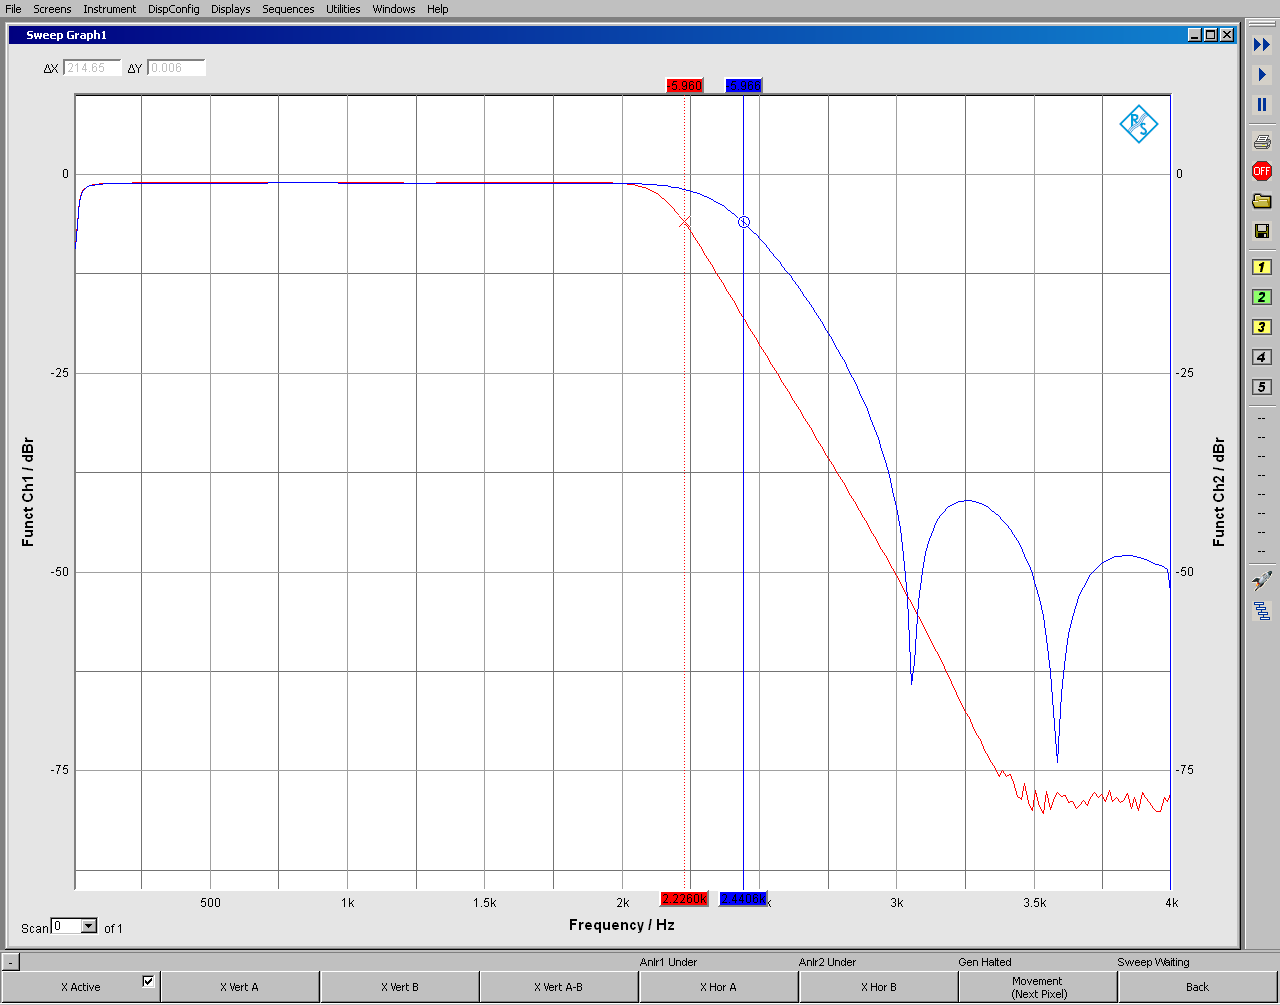
\includegraphics[width=0.8\linewidth]{Bilder/EllipCheby}
		\caption{Blau: Elliptisches IIR TP-Filter | Rot: Chebychev IIR TP-Filter}
		\label{fig:EllipCheby}
	\end{figure}
	
\noindent Der linke Ausgang lieferte das mit einem elliptischen TP-Filter gefilterte Eingangssignal (blau), der rechte Ausgang lieferte das mit einem Chebychev-TP-Filter gefilterte Eingangssignal (rot). Ein Frequenzsweep von 0 .. 4kHz wurde für die Messungen durchgeführt. Die Filterrealisierung geschah jeweils über k kaskadierter Biquads zweiter Ordnung. Für das elliptische Filter war k = 2, für Chebychev war k = 3.

\subsubsection{Attachement G}
\noindent Die Unterschiede in der Implementierung ergeben sich eindeutig:
\begin{itemize}
	\item Elliptisches Filter: 2 Stufen, somit 2 Biquads
	\item Chebychev Filter: 3 Stufen, somit 3 Biquads
\end{itemize}
\noindent Der Rechenaufwand des Chebychev Tiefpasses ist folglich anderthalb mal so groß wie der des Elliptischen Tiefpasses.

\clearpage

\subsection{Hochpass - Tiefpass - Weichenfilter}
\noindent Nun wurde auf dem linken Ausgangskanal das mit einem elliptischen Tiefpass gefilterte Eingangssignal ausgegeben, auf dem rechten Ausgangskanal wurde das mit einem elliptischen Hochpass gefilterte Eingangssignal ausgegeben.

\begin{figure}[h]
	\centering
	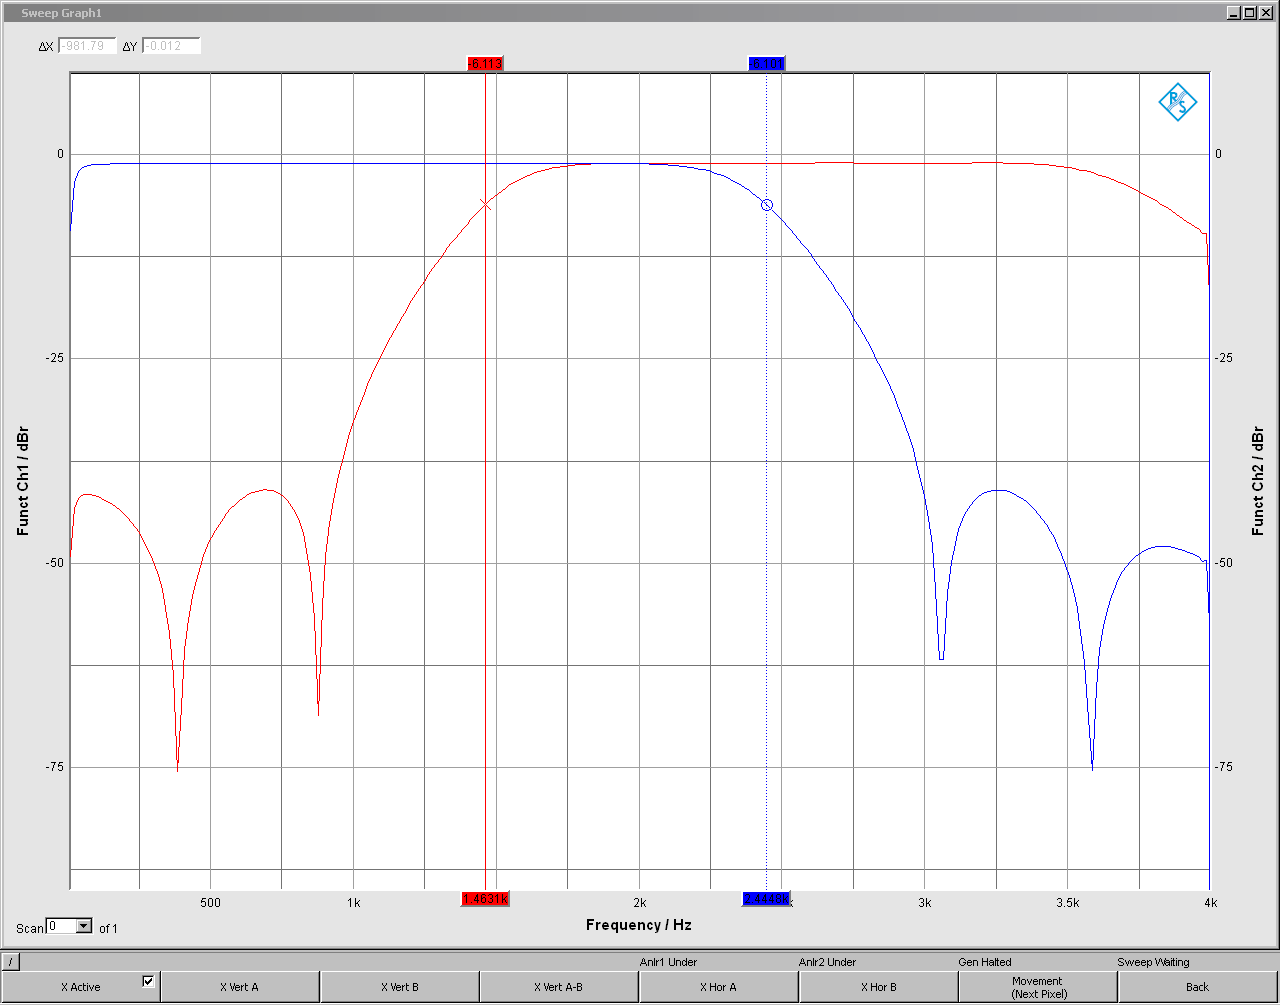
\includegraphics[width=0.7\linewidth]{Bilder/EllipTPHP}
	\caption{Blau: elliptischer Tiefpass | Rot: elliptischer Hochpass}
	\label{fig:EllipTPHP}
\end{figure}

\clearpage

\subsection{Modifiziertes elliptisches Tiefpassfilter}
\subsubsection{Attachement H}
\noindent Durch die Verwendung der doppelten Verzögerungszeit $|T| \rightarrow |2T|$ verschiebt sich der Frequenzgang des Tiefpassfilter.

\begin{figure}[h]
\centering
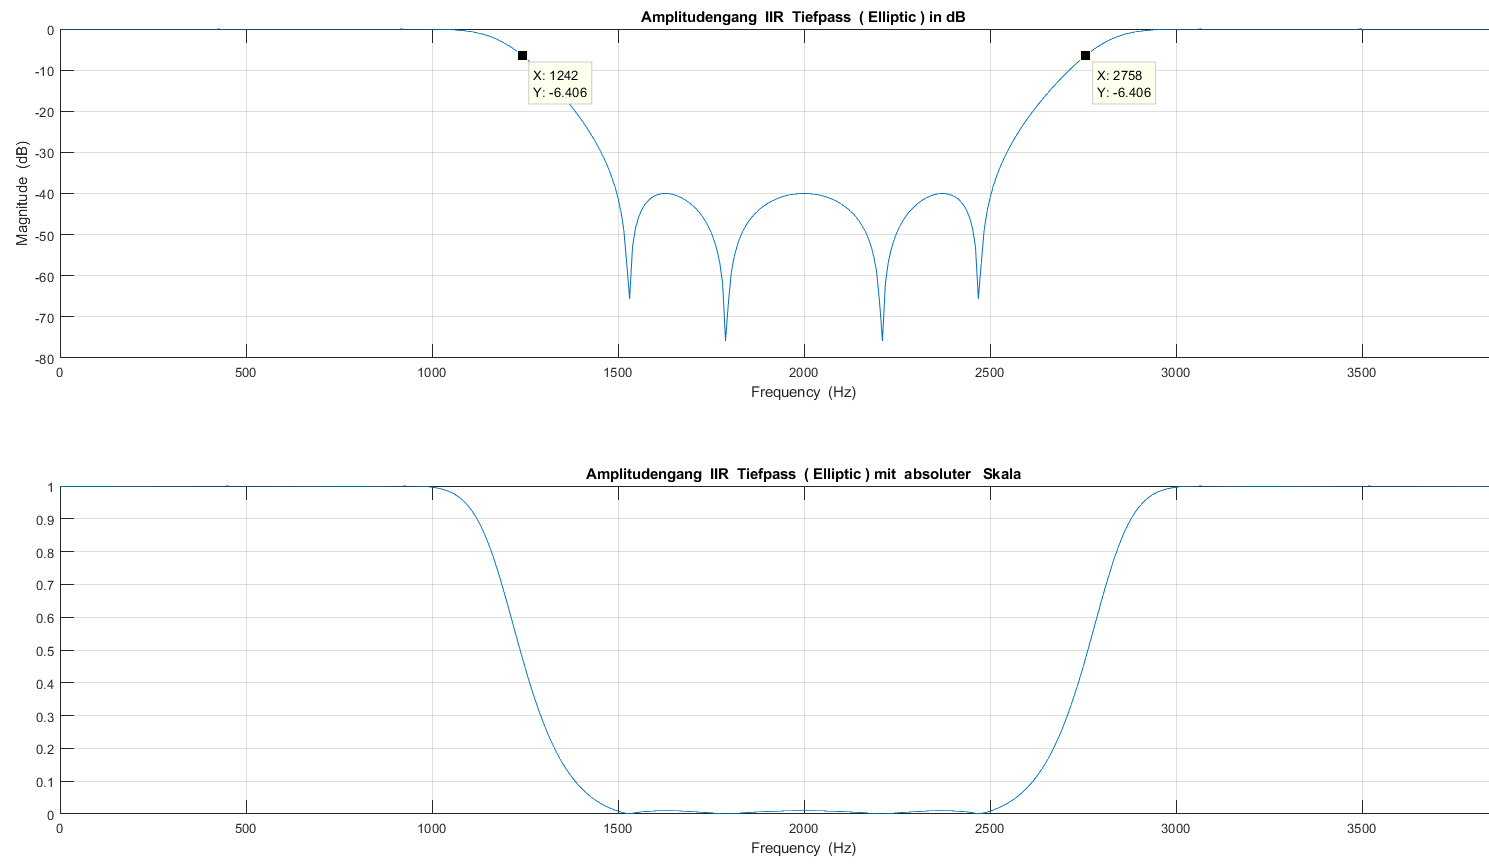
\includegraphics[width=0.7\linewidth]{./Bilder/Attachment_H_ELLIP_STOP}
\caption{Amplitudengang Bandsperre $T \rightarrow 2T$}
\label{fig:Attachment_H_ELLIP_STOP}
\end{figure}

\noindent Durch diese Modifikation wird aus dem Tiefpass eine Bandsperre. Eine weitere Erklärung ist in Kapitel Attachement K herleitet.



\subsubsection{Attachement J}

\begin{figure}[h]
\centering
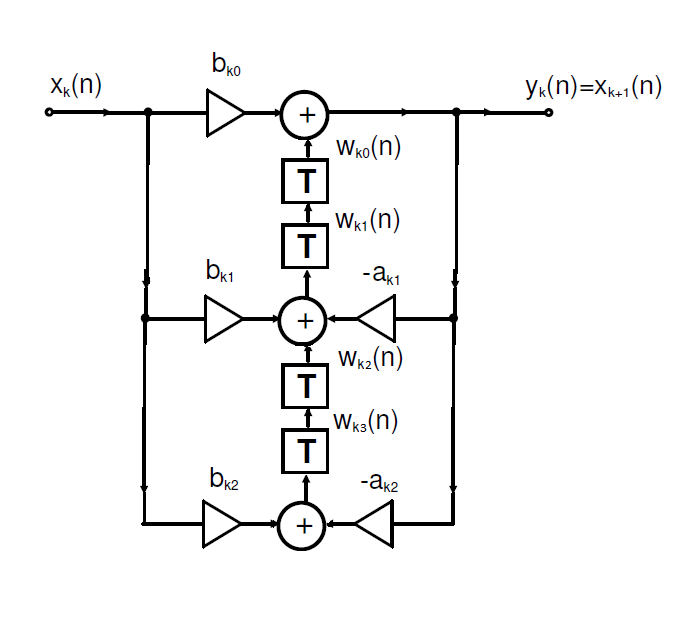
\includegraphics[width=0.7\linewidth]{Bilder/Biquad2T}
\caption{Verwendete Biquad-Sektion mit 2 Verzögerungen}
\label{fig:Biquad2T}
\end{figure}

\noindent Es wurde jeweils eine weitere Verzögerung implementiert. Es ergibt sich in C-Syntax:\\
$W_{k0}(n)=W_{k1}(n)$\\
$W_{k1}(n)=b_{k1}*x_k(n))+y_k(n)*(-a_{k1})+W_{k2}(n)$\\
$W_{k2}(n)=W_{k3}(n)$\\
$W_{k3}(n)=b_{k2}*x_k(n)+y_k(n)*(-a_{k2})$

\clearpage

\subsubsection{Attachement K}

	\begin{figure}[h]
		\centering
		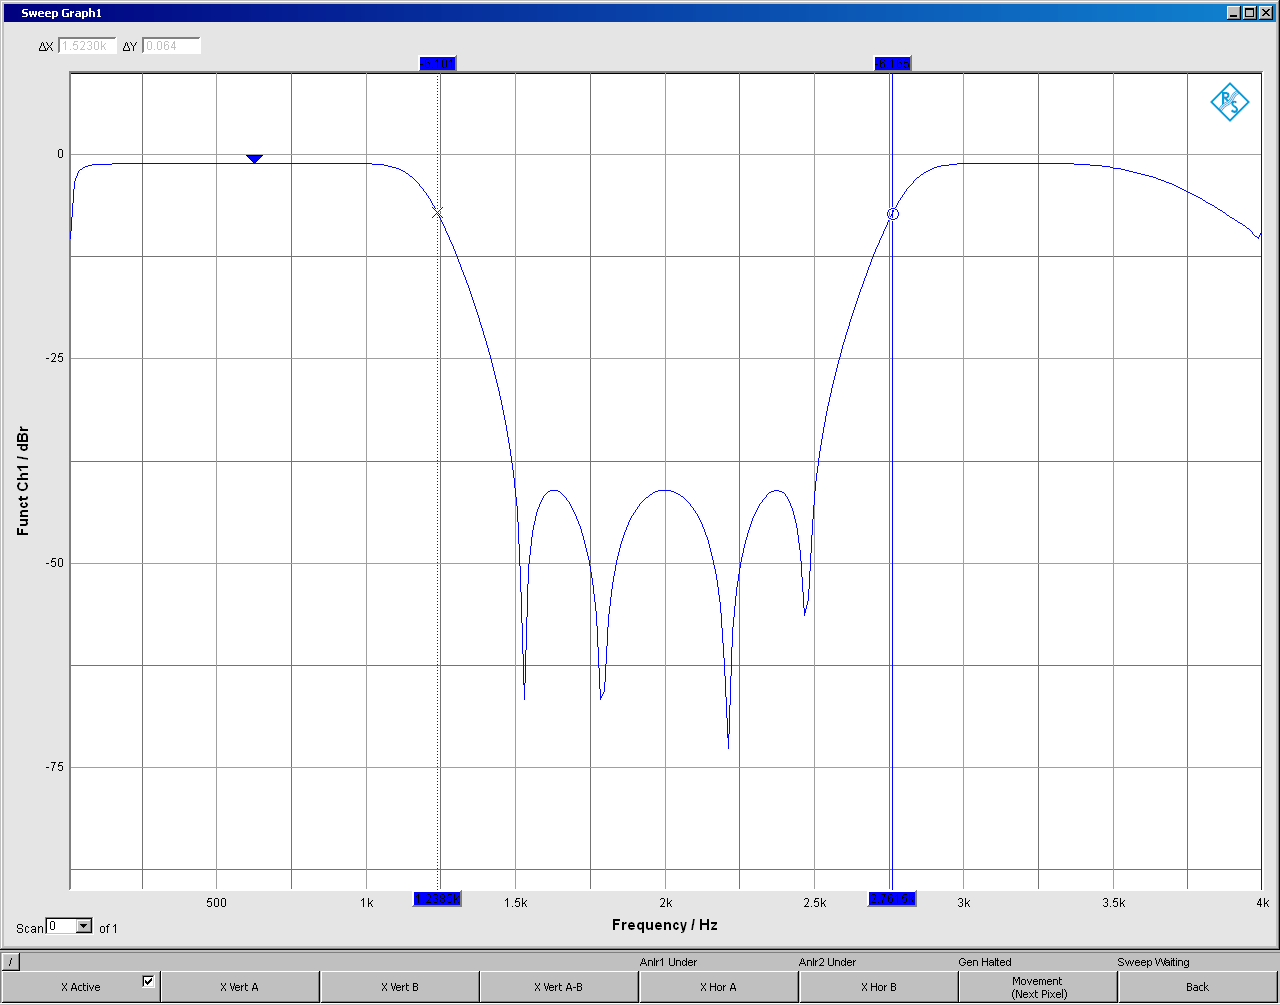
\includegraphics[width=0.7\linewidth]{Bilder/ellip2T}
		\caption{Frequenzgang modifiziertes Tiefpassfilter $|T| \rightarrow |2T|$}
		\label{fig:ellip2T}
	\end{figure}
	
\noindent Durch die Verwendung der doppelten Verzögerungszeit $|T| \rightarrow |2T|$ verschiebt sich der Frequenzgang des Tiefpasses. Der gleiche Effekt würde bei der Halbierung der Abtastfrequenz des DSPs auftreten. Der sich periodisch wiederholende Frequenzgang des Filters ist nun dichter zusammengerückt. Wir sehen auf der Abbildung den um $\frac{f_s}{2}$ gespiegelten Frequenzgang. 
